\section{Getting started}

Here's a quick walk-through of the package. Here, we will
a) build a model of an RNA multiple alignment using
         \prog{cmbuild};
b) use that model to search for new homologs using
         \prog{cmsearch};
and c) use that model to align new sequences, and create a 
         new multiple alignment, using \prog{cmalign}.

We'll use the following files, all of which are in the \prog{intro/}
subdirectory of the distribution:

  \begin{sreitems}{tutorial.sto}
  \item[\prog{tutorial.sto}] A multiple alignment of five tRNA
       sequences. This file is a simple example of \emph{Stockholm
       format} that \software{infernal} uses for structurally-annotated alignments.
  \item[\prog{tutorial.db}]  A tiny sequence ``database''; a 300 nt sequence
       that contains a tRNA. The file is
       in FASTA format, which \software{infernal} uses for unaligned sequence
       data.
  \item[\prog{tutorial.big.db}]  A larger 300,000 nt sequence database; 
       with the same tRNA as in \prog{tutorial.db}. Used to
       demonstrate HMM filtered search. 
  \item[\prog{tutorial.fa}] The same sequences as in \prog{tutorial.sto}, plus
       one more tRNA with an internal deletion (to demonstrate local alignment),
       in unaligned FASTA format.
  \end{sreitems}

\subsection{Format of a simple input RNA alignment file}

Look at the alignment file \prog{tutorial.sto} in the \prog{intro/}
subdirectory of the \software{infernal} distribution. It is shown
below, with a secondary structure of the first sequence shown to the
right for reference (yeast Phe tRNA, labeled as ``tRNA1'' in the
file):

\vspace{1em}
\begin{minipage}{4.7in}
\begin{sreoutput}[xleftmargin=0em]
# STOCKHOLM 1.0

tRNA1             GCGGAUUUAGCUCAGUUGGG.AGAGCGCCAGACUGAAGAUCUGGAGGUCC
tRNA2             UCCGAUAUAGUGUAAC.GGCUAUCACAUCACGCUUUCACCGUGGAGA.CC
tRNA3             UCCGUGAUAGUUUAAU.GGUCAGAAUGGGCGCUUGUCGCGUGCCAGA.UC
tRNA4             GCUCGUAUGGCGCAGU.GGU.AGCGCAGCAGAUUGCAAAUCUGUUGGUCC
tRNA5             GGGCACAUGGCGCAGUUGGU.AGCGCGCUUCCCUUGCAAGGAAGAGGUCA
#=GC SS_cons      <<<<<<<..<<<<.........>>>>.<<<<<.......>>>>>.....<

tRNA1             UGUGUUCGAUCCACAGAAUUCGCA
tRNA2             GGGGUUCGACUCCCCGUAUCGGAG
tRNA3             GGGGUUCAAUUCCCCGUCGCGGAG
tRNA4             UUAGUUCGAUCCUGAGUGCGAGCU
tRNA5             UCGGUUCGAUUCCGGUUGCGUCCA
#=GC SS_cons      <<<<.......>>>>>>>>>>>>.
//
\end{sreoutput}
\end{minipage}
\begin{minipage}{1.5in}
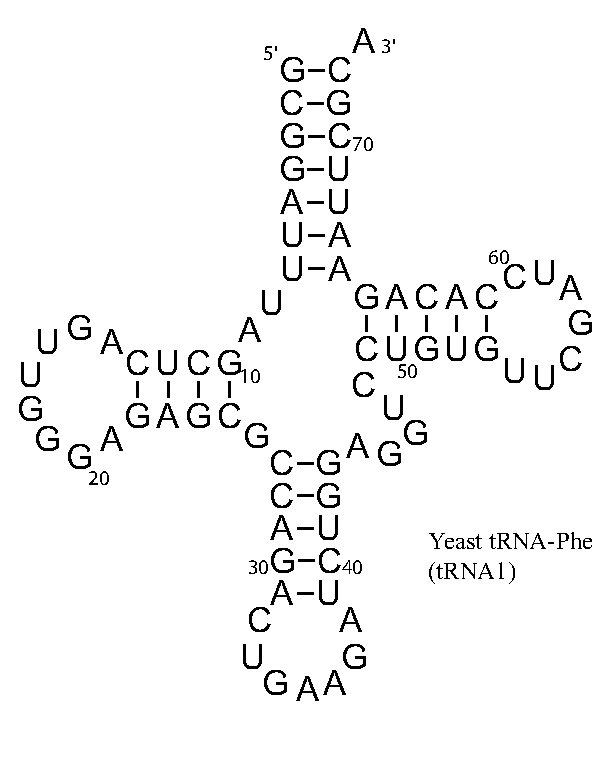
\includegraphics[scale=0.4]{Figures/trna1-DF6280}
\end{minipage}
\vspace{1em}

This is a simple example of a multiple RNA sequence alignment with
secondary structure annotation, in \emph{Stockholm format}. Stockholm
format, the native alignment format used by \software{hmmer} and
\software{infernal} and the \database{Pfam} and \database{Rfam}
databases, is documented in detail later in the guide.

For now, what you need to know about the key features of the input file is:
\begin{itemize}
\item The alignment is in an interleaved format, like other
common alignment file formats such as \software{clustalw}.
Lines consist of a name, followed by an aligned sequence;
long alignments are split into blocks separated by blank lines.
\item Each sequence must have a unique name. (This is important!)
\item For residues, any one-letter IUPAC nucleotide code is accepted,
      including ambiguous nucleotides. Case is ignored; residues
      may be either upper or lower case.
\item Gaps are indicated by the characters ., \_, -, or \verb+~+.
      (Blank space is not allowed.)
\item A special line starting with {\small\verb+#=GC SS_cons+} indicates
      the secondary structure consensus. Gap characters annotate
      unpaired (single-stranded) columns. Base pairs are indicated
      by any of the following pairs: \verb+<>+, \verb+()+, \verb+[]+,
      or \verb+[]+. No pseudoknots are allowed; the
      open/close-brackets notation is only unambiguous for strictly
      nested base-pairing interactions.
\item The file begins with the special tag line
      {\small\verb+# STOCKHOLM 1.0+}, and ends with {\small\verb+//+}.
\end{itemize}

\subsection{Building a model with \prog{cmbuild}}

To build a model from this alignment, do:

\user{cmbuild my.cm tutorial.sto}

Almost instantly, \prog{cmbuild} reads in the alignment, constructs a
model, and saves that model to the new file \prog{my.cm}. It is a
convention to use the \prog{.cm} suffix for model files; CM stands for
``covariance model'', another name for the profile SCFG architecture
used by \software{infernal} \cite{Eddy94}.

The output \prog{cmbuild} contains information about the size of your
input alignment (in aligned columns and \# of sequences), and about
the size of the resulting model. You don't need to understand this to
use the model, so for now we'll skip describing the output. 

The result, the model file in \prog{my.cm} is a text file. You can
look at it (e.g. \prog{> more my.cm}) if you like, but it isn't really
designed to be human-interpretable. You can treat \prog{.cm} files as
compiled models of your RNA alignment.

\newpage
\subsection{Searching a sequence database with \prog{cmsearch}}

You can use your model to search for new homologues of your RNA
family. The file \prog{tutorial.db} contains an example sequence
``database'': one 300 nt sequence, with yeast tRNA-Phe embedded at
position 101\ldots173. To search it, do:

\user{cmsearch my.cm tutorial.db}

\prog{cmsearch} now searches both strands of each sequence in the
target database, and returns alignments for high scoring hits.  In
this case, it returns one hit:

\begin{sreoutput}
CM 1: tutorial.1
CM lambda and K undefined -- no statistics
Using CM score cutoff of 0.00
>example

  Plus strand results:

 Query = 1 - 72, Target = 101 - 173
 Score = 65.96, GC =  53

           (((((((,,<<<<___.____>>>>,<<<<<_______>>>>>,,,,,<<<<<_______
         1 gccgacaUaGcgcAgu.GGuAgcgCgccagcuUgaaaagcuggAGguccgggGUUCgAuu 59      
           GC:+A::UAGC:CAGU GG AG:GCGCCAG:+UGAA A:CUGGAGGUCC:G:GUUCGAU 
       101 GCGGAUUUAGCUCAGUuGGGAGAGCGCCAGACUGAAGAUCUGGAGGUCCUGUGUUCGAUC 160     

           >>>>>))))))):
        60 Ccccgugucggca 72      
           C:C:G::U+:GCA
       161 CACAGAAUUCGCA 173     


//
Fin
\end{sreoutput}

The first line gives the name of the CM (this can be defined in the
input Stockholm alignment file or as an option to \prog{cmbuild}, as
described later).
The next two lines give information on E-value statistics, which were
turned off in our example search (more on this later).  Next comes
the results section, the name of each target sequence in the target
database is given starting with a \prog{$>$}, in this case there is
only one: \prog{example}. Next, all the hits to the top (Watson)
strand of \prog{example} are given, in this example there is a single hit from
position 101 to 173 with a score of 65.96 bits. As discussed next,
E-value statistics can give an estimate of the significance of bit
scores. We have not rigorously tested our implementation of E-values,
so by default E-values are not calculated. Larger bit scores
scores are better. As a rough guide, scores greater than the log (base
two) of the target database size are significant.  Here, given a 600
nt target (300 nt $\times$ 2 strands), scores over 9-10 bits are
significant - so a score of 65.96 is a good hit.

%Hits are numbered starting from 0. This one shows hit 0, from position
%101 to 173 on the sequence named ``example'', with a score of 22.29
%bits. There are no E-value statistics yet in \software{infernal}, so
%this score is all you have to go by to determine significance of a
%hit.  Larger scores are better. As a rough guide, scores greater than
%the log (base two) of the target database size are significant.  Here,
%given a 600 nt target (300 nt $\times$ 2 strands), scores over 9-10
%bits are significant - so a score of 22.29 is a good hit. 

The alignment is shown in a BLAST-like format, augmented by secondary
structure annotation. 

The top line shows the predicted secondary structure of the target
sequence. The format is a little fancier and more informative than the
simple least-common-denominator format we used in the input alignment
file. It's designed to make it easier to ``see'' the secondary
structure by eye. The format is described in detail later; for now,
here's all you need to know. Base pairs in simple stem loops are
annotated with \verb+<>+ characters. Base pairs enclosing
multifurcations (multiple stem loops) are annotated with \verb+()+,
such as the tRNA acceptor stem in this example. In more complicated
structures, \verb+[]+ and \verb+{}+ annotations also show up, to
reflect deeper nestings of multifurcations. For single stranded
residues, \_ characters mark hairpin loops; \- characters mark
interior loops and bulges; , characters mark single-stranded residues
in multifurcation loops; and : characters mark single stranded
residues external to any secondary structure. Insertions relative to
this consensus are annotated by a \verb+.+ character.

The second line shows that consensus of the query model. The highest
scoring residue sequence is shown. Upper case residues are highly
conserved. Lower case residues are weakly conserved or unconserved.

The third line shows where the alignment score is coming from. For a
consensus base pair, if the observed pair is the highest-scoring
possible pair according to the consensus, both residues are shown in
upper case; if a pair has a score of $\geq 0$, both residues are
annotated by : characters (indicating an acceptable compensatory base
pair); else, there is a space, indicating that a negative contribution
of this pair to the alignment score. For a single-stranded consensus
residue, if the observed residue is the highest scoring possibility,
the residue is shown in upper case; if the observed residue has a
score of $\geq 0$, a \verb@+@ character is shown; else there is a
space, indicating a negative contribution to the alignment score.

Finally, the fourth line is the target sequence.

Let's repeat this example search, now with E-values. When run with the
\prog{-E} option, \prog{cmsearch} estimates the E-value of each hit
found. This is
computed by sampling 1000 random sequences and determining the bit
score of the best hit within each sequence, these scores are fit to a
Gumbel distribution. The search is then carried out, and the Gumbel
distribution is used to estimate the significance of the bit scores of
the hits found. This procedure used by \prog{cmsearch} is very
similar to that described for the \software{RSEARCH} program in
\cite{KleinEddy03}. Because using E-values requires searching
1000 random sequences, it takes quite a bit longer than a regular
search. To repeat the search saving all hits with E-values of 10 or
less, do:

\user{cmsearch -E 10 my.cm tutorial.db}

{\samepage
\begin{sreoutput}
CM 1: tutorial.1
CM statistics calculated with simulation of 1000 samples of length 180
Random seed: 1177592728
No partition points
Using CM E cutoff of 10.00

>example

  Plus strand results:

 Query = 1 - 72, Target = 101 - 173
 Score = 65.96, E = 6.27e-12, P = 6.27e-12, GC =  53

           (((((((,,<<<<___.____>>>>,<<<<<_______>>>>>,,,,,<<<<<_______
         1 gccgacaUaGcgcAgu.GGuAgcgCgccagcuUgaaaagcuggAGguccgggGUUCgAuu 59      
           GC:+A::UAGC:CAGU GG AG:GCGCCAG:+UGAA A:CUGGAGGUCC:G:GUUCGAU 
       101 GCGGAUUUAGCUCAGUuGGGAGAGCGCCAGACUGAAGAUCUGGAGGUCCUGUGUUCGAUC 160     

           >>>>>))))))):
        60 Ccccgugucggca 72      
           C:C:G::U+:GCA
       161 CACAGAAUUCGCA 173     


//
Fin
\end{sreoutput}
}

The output tells us that the E-value is $6.27e-12$, this is the number
of hits we expect to find with a bit score of 65.96 or better if we
were searching a database of random sequence of length 300.

\subsection{Accelerating \prog{cmsearch}}
The \prog{cmsearch} program is very slow, and several techniques have
been developed for acceleration. We'll briefly discuss two here (for
more information see the \prog{cmsearch} man pages at the end of this
guide).

The first acceleration strategy is called query-dependent banding
(QDB). Briefly, this technique precalculates regions of the dynamic programming
matrix that have very low probability before the search, and skips these
regions during the search \cite{NawrockiEddy07}. 
By default, QDB is on in \prog{cmsearch}, you can turn it off with the
\prog{--noqdb} option. QDB offers about a four-fold speedup for an
average RNA family, with very little impact on sensitivity. In
general, the longer the average sequence length of an RNA family, the
greater the acceleration achieved by using QDB.

The second acceleration technique is filtering the target database
with a profile HMM, and using the expensive CM based search on only
subsequences that receive high HMM scores. This was pioneered by Zasha
Weinberg and Larry Ruzzo at the University of Washington
\cite{WeinbergRuzzo04,WeinbergRuzzo04b,WeinbergRuzzo06}. Here we
consider two of their techniques for constructing a profile HMM. The
first builds a ``rigorous filter'' that is guaranteed to find all CM
hits above a certain threshold. We have incorporated Weinberg's
implementation of ``rigorous filters'' into \software{infernal} but
not within the \prog{cmsearch} program. (For details see the file
\prog{rigfilters\_doc.html} in the \prog{documentation/userguide}
subdirectory of the top level \prog{infernal} directory.) The second
HMM filtering method involves a maximum likelihood (ML) HMM that is
not guaranteed to find all hits, but is more practical than rigorous
filters for many RNA families. We have implemented a version of ML
HMMs in \software{infernal}, which we call these CM Plan 9 HMMs (CP9
HMMs), to distinguish them from the Plan 7 HMMs of \software{hmmer}.
CP9 HMMs can be used to accelerate \prog{cmsearch} using the
\prog{--hmmfilter} option, as well as to accelerate \prog{cmalign} as
discussed later in this guide.  We still consider our implementation
of the CP9 HMM filtering technique experimental, so it is not on by
default.  When the \prog{--hmmfilter} option is enabled, E-values are
calculated for the CP9 HMM in the same manner that CM E-values are
calculated, except this time each of the 1000 random sequences is
searched with the HMM, so it is much quicker. The database is then
searched with the CP9 HMM and high scoring HMM hits with E-values of
500 or less (along with some flanking sequence) are searched again with
the CM.  The default E-value threshold of 500 can be changed with the
\prog{--hmmE} option. Also, a bit score threshold can be set instead
of an E-value threshold with the \prog{--hmmT} option.  Here's an
example searching a larger sample database called
\prog{tutorial.big.db}, which is 300,000 nt and still has the tRNA
from position 101 to 173:

\user{cmsearch --hmmfilter my.cm tutorial.big.db}

This search finds the real tRNA and takes about 45 seconds on my
machine. The same search without HMM filtering and with the \prog{--time}
option to print timings can be run with:

\user{cmsearch --time my.cm tutorial.big.db}

On my machine, this non-filtered search takes about 8 minutes, meaning
the HMM gave us about a 10-fold speedup. This speedup will increase 
for RNA families with longer sequence lengths, or if you lower the
E-value cutoff with \prog{--hmmE}. The speedup comes at a
cost to sensitivity though, and we haven't
rigorously tested this to our satisfaction. This is the main reason
this option is not on by default. There are more options related to
HMM filtering for \prog{cmsearch} discussed in the man pages at the
end of this guide.

\subsection{Creating new multiple alignments with \prog{cmalign}}

You can also use a model to structurally align any number of new RNA
sequences to your consensus structure. This is how the \database{Rfam}
database is constructed: we start with ``seed'' alignment, build a CM
of it, and use that CM to align all known members of the sequence
family and create a ``full'' alignment. This allows us to maintain
representative seed alignments that are stable and small enough to be
human-curated, while still being able to automatically incorporate and
align all homologues detected in the rapidly growing public sequence
databases.

An example of some unaligned tRNA sequences are in the file
\prog{tutorial.fa}. (In fact, these are the same sequences that are in
\prog{tutorial.sto}, reformatted into unaligned FASTA format; plus a
new sequence, tRNA6, which was created by deleting some residues out
of the middle of tRNA1. tRNA6 will be used a little later to
demonstrate local alignment.)

To align these sequences to the model we made in \prog{my.cm}, do:

\user{cmalign my.cm tutorial.fa}

This results in an alignment that looks like:

{\samepage
\begin{sreoutput}
# STOCKHOLM 1.0
#=GF AU    Infernal 0.72

tRNA1             GCGGAUUUAGCUCAGUuGGG.AGAGCGCCAGACUGAAGAUCUGGAGGUCC
tRNA2             UCCGAUAUAGUGUAAC.GGCuAUCACAUCACGCUUUCACCGUGGAGA-CC
tRNA3             UCCGUGAUAGUUUAAU.GGUcAGAAUGGGCGCUUGUCGCGUGCCAGA-UC
tRNA4             GCUCGUAUGGCGCAGU.GGU.AGCGCAGCAGAUUGCAAAUCUGUUGGUCC
tRNA5             GGGCACAUGGCGCAGUuGGU.AGCGCGCUUCCCUUGCAAGGAAGAGGUCA
tRNA6             GCGGAUUUAGCUCAGUuGGG.AGAGCGC------CAGAC----GAGGUCC
#=GC SS_cons      (((((((,,<<<<___.___._>>>>,<<<<<_______>>>>>,,,,,<
#=GC RF           gccgacaUaGcgcAgu.GGu.AgcgCgccagcuUgaaaagcuggAGgucc

tRNA1             UGUGUUCGAUCCACAGAAUUCGCA
tRNA2             GGGGUUCGACUCCCCGUAUCGGAG
tRNA3             GGGGUUCAAUUCCCCGUCGCGGAG
tRNA4             UUAGUUCGAUCCUGAGUGCGAGCU
tRNA5             UCGGUUCGAUUCCGGUUGCGUCCA
tRNA6             UGUGUUCGAUCCACAGAAUUCGCA
#=GC SS_cons      <<<<_______>>>>>))))))):
#=GC RF           gggGUUCgAuuCcccgugucggca
//
\end{sreoutput}
}

In the aligned sequences, a \verb@.@ character indicates an inserted
column relative to consensus; the \verb@.@ character is an alignment
pad. A \verb+-+ character is a deletion relative to consensus.

The symbols in the consensus secondary structure annotation line have
the same meaning that they did in a pairwise alignment from
\prog{cmsearch}.

The {\small\verb+#=GC RF+} line is \emph{reference
annotation}. Non-gap characters in this line mark consensus columns;
\prog{cmalign} uses the residues of the consensus sequence here, with
upper case denoting strongly conserved residues, and lower case
denoting weakly conserved residues. Gap characters (specifically, the
\verb+.+ pads) mark insertions relative to consensus. As described
below, \prog{cmbuild} is capable of reading these RF lines, so you can
specify which columns are consensus and which are inserts (otherwise,
\prog{cmbuild} makes an automated guess, based on the frequency of
gaps in each column).

If you want to save the alignment to a file, you can use the \prog{-o}
option:

\user{cmalign -o my.sto my.cm tutorial.fa}

We'll use this \prog{my.sto} alignment file in an upcoming section.

\subsection{Accelerating \prog{cmalign}}
Earlier in this guide, we described the use of CM Plan 9 HMMs (CP9
HMMs) as filters to accelerate \prog{cmsearch} using the
\prog{--hmmfilter} option. CP9 HMMs can also be used to accelerate CM
alignment. The basic idea is to first align each sequence to the CP9
HMM and to use that alignment to derive constraints, which we call
bands, for the more
computationally expensive CM alignment. These bands are then
applied during CM alignment, reducing the time necessary for
alignment. This technique can be enabled with the \prog{--hbanded}
option to \prog{cmalign}. Here's an
example: 

\user{cmalign --hbanded my.cm tutorial.fa}

You may notice that this time the program runs a bit
quicker than before. It's almost imperceptible here, but for large RNAs the
difference is significant. For example, alignment of small subunit ribosomal
RNA (SSU rRNA) sequences (which are roughly 1500 nucleotides) using
the \prog{--hbanded} option takes close to one second for one sequence, whereas
non-banded alignment takes several minutes. Importantly, using the HMM banded
technique sacrifices the guarantee that the optimal alignment will be
found, but our tests suggests this happens very rarely for non-local
alignment (these tests were done using the \prog{cmscore} program).
However, we have not rigorously tested the \prog{--hbanded} option for local
alignment. More information on HMM banded alignment can be found in
the \prog{cmalign} and \prog{cmscore} man pages at the end of this guide.

\subsection{Using optional annotation to completely specify model architecture
to \prog{cmbuild}}

\prog{cmbuild} needs to know two things to convert your alignment into
a profile SCFG.

First, it needs to know the consensus secondary structure. It reads
this from the {\small\verb+#=GC SS_cons+} line, as described
above. This annotation is mandatory.

It also needs to know which columns are consensus, and which columns
are insertions relative to consensus. By default, it will determine
this by a simple rule: if a column contains more than a certain
fraction of gap characters (default $>$50\%), the column is called an
insertion. This may not be what you want; for instance, maybe you are
trying to iteratively build models based on larger and larger numbers
of sequences (based on an \database{Rfam} seed, say), but you don't
want the curated consensus model architecture to change just because
you added some new sequences to the alignment.

You can optionally override that default and specify the complete
architecture of the model, using both a {\small\verb+#=GC SS_cons+}
structure annotation line and a {\small\verb+#=GC RF+} reference
column annotation line.  To do this, you use the \prog{--rf} flag to
\prog{cmbuild}.

For example, to build a model called \prog{second.cm} from
\prog{my.sto} that has the same architecture as \prog{my.cm}, you
would do:

\user{cmbuild --rf second.cm my.sto}

Since \prog{cmalign} leaves an RF line on the alignments it generates,
the \prog{--rf} option allows you to propagate your consensus
structure into new, larger alignments. The RF line is also handy when
you want the model's coordinate system to be the same as a canonical,
well-studied single sequence: you can simply use that sequence as the
RF line, or manually create any consensus coordinate system you like.
(This is the origin of RF as the ``reference line'', e.g.\ giving a
reference coordinate system.) The only thing that matters in the RF
line is nongap versus gap characters: the line can be as simple as x's
marking consensus columns, \verb+.+'s for insert columns.

\subsection{Using local alignment in \prog{cmsearch} and \prog{cmalign}}

The examples above required the entire model to match a subsequence of
the target: so-called \emph{glocal} alignment (global with respect to
the query model, local with respect to the target sequence). But in
many cases, a homologous RNA structure has undergone enough changes
that parts of its structure cannot be aligned to the
onsensus. \emph{Local} alignment, in which only part of the query
model needs to match the target to detect a hit, can be a more
sensitive searching strategy.

In primary sequence alignment, local alignment means an alignment of
two subsequences of the query and target. In aligning a query RNA
structure to a target sequence, local alignment means starting and
ending at points inside the query structure -- which, when you map
that idea onto linear sequence, means an alignment that may consist of
more than one discontinuous subsequence. We'll demonstrate this by
example for now, and describe local alignment is described in detail
later.  For the purposes of the tutorial, all you really need to know
is how to activate it. It is not the default behavior for either
\prog{cmsearch} or \prog{cmalign}.

Local alignment is activated for \prog{cmsearch} by using the
\prog{--local} option. For example:

\user{cmsearch --local my.cm tutorial.fa}

Look at the first alignment for the target sequence tRNA6 (the second
to last alignment in the output): 

\begin{sreoutput}
>tRNA6

  Plus strand results:

 Query = 1 - 72, Target = 1 - 63
 Score = 44.94, GC =  55

           (((((((,,<<<<___.____>>>>,<~~~~~~>,,,,,<<<<<_______>>>>>))))
         1 gccgacaUaGcgcAgu.GGuAgcgCgc*[15]*gAGguccgggGUUCgAuuCcccguguc 68      
           GC:+A::UAGC:CAGU GG AG:GCGC      GAGGUCC:G:GUUCGAU C:C:G::U+
         1 GCGGAUUUAGCUCAGUuGGGAGAGCGC*[ 5]*GAGGUCCUGUGUUCGAUCCACAGAAUU 59      

           ))):
        69 ggca 72      
           :GCA
        60 CGCA 63      
\end{sreoutput}

The \verb+*[15]*+ and \verb+*[5]*+ in the query and target,
respectively, indicate that 15 consensus residues and 5 target
residues were left unaligned; the target does not appear to have the
consensus structure in this region. (No kidding, since I made the
tRNA6 example sequence by deleting part of the anticodon stem.)  The
structure annotation line is marked with \verb+~~~~~~+ to indicate the
gap in the alignment, and to distinguish local alignment induced gaps
from normal insertions (which are marked with \verb+.+ characters).

You can activate local alignment in \prog{cmalign} with the \prog{-l}
option:

\user{cmalign -l my.cm tutorial.fa}

This results in the following alignment:
\footnote{The discontinuity of structural local alignment presents a
quandary for representing multiple alignments. On the one hand, you
might not want to even show the unaligned target residues in the gap
(e.g., cagac) -- they aren't aligned to the model. On the other hand,
you sort of expect that if you pull an RNA sequence out of a multiple
alignment, it represents a true subsequence of a larger sequence, not
a concatenation of disjoint subsequences -- you'd at least like some
indication of where some residues have gone missing. One option would
be to leave a *[5]* in the gap, as in the pairwise
representation; but one of the nice properties of Stockholm format is
that it's easy to interconvert it to other alignment formats just by
stripping off everything by the name/sequence part of the alignment,
and sticking non-sequence characters like *[5]* in the
alignment would prevent that.}

{\samepage
\begin{sreoutput}
# STOCKHOLM 1.0
#=GF AU    Infernal 0.72

tRNA1             GCGGAUUUAGCUCAGUuGGG.AGAGCGCCAGACUGAAGA.....UCUGGA
tRNA2             UCCGAUAUAGUGUAAC.GGCuAUCACAUCACGCUUUCAC.....CGUGGA
tRNA3             UCCGUGAUAGUUUAAU.GGUcAGAAUGGGCGCUUGUCGC.....GUGCCA
tRNA4             GCUCGUAUGGCGCAGU.GGU.AGCGCAGCAGAUUGCAAA.....UCUGUU
tRNA5             GGGCACAUGGCGCAGUuGGU.AGCGCGCUUCCCUUGCAA.....GGAAGA
tRNA6             GCGGAUUUAGCUCAGUuGGG.AGAGCGC-----------cagac----GA
#=GC SS_cons      (((((((,,<<<<___.___._>>>>,<<<<<_______~~~~~>>>>>,
#=GC RF           gccgacaUaGcgcAgu.GGu.AgcgCgccagcuUgaaaa~~~~~gcuggA

tRNA1             GGUCCUGUGUUCGAUCCACAGAAUUCGCA
tRNA2             GA-CCGGGGUUCGACUCCCCGUAUCGGAG
tRNA3             GA-UCGGGGUUCAAUUCCCCGUCGCGGAG
tRNA4             GGUCCUUAGUUCGAUCCUGAGUGCGAGCU
tRNA5             GGUCAUCGGUUCGAUUCCGGUUGCGUCCA
tRNA6             GGUCCUGUGUUCGAUCCACAGAAUUCGCA
#=GC SS_cons      ,,,,<<<<<_______>>>>>))))))):
#=GC RF           GguccgggGUUCgAuuCcccgugucggca
//
\end{sreoutput}
}

Note how the local alignment is represented for tRNA6. The deleted
consensus columns are marked by - characters. The unaligned
``insertion'' is shown in its own columns; those columns are again
marked with \verb+~+ characters in the consensus secondary structure
annotation and the reference (RF) annotation lines.

%\subsection{An important limitation to \prog{cmsearch}: the -W option}

%\prog{cmsearch} implements a ``scanning CYK'' dynamic programming
%algorithm \cite{Durbin98} that looks for high-scoring alignments of
%the structural model to any subsequence of the target sequence. It
%works even if the target sequence is very large (e.g.\ a whole
%chromosome) -- though it is slow, like all SCFG algorithms. An
%important feature of the scanning CYK algorithm is that it needs to
%know the \emph{maximum length} of an aligned target subsequence, e.g.
%the size of its scanning window on the target sequence.

%By default, the scanning window is calculated by \prog{cmbuild} and
%stored in the model. The calculation is fairly rigorous, based on the
%expected probability density over possible lengths
%\cite{NawrockiEddy07}. The result will almost certainly be fine for
%your purposes.  However, you can override it and set the scanning
%window width yourself to \verb+<n>+ with the \prog{-W <n>} option.
%
%Even if the target RNA is larger than the scanning window, there is
%some chance of finding part of it -- particularly in combination with
%local alignment (\prog{--local}), which explicitly allows partial
%matches to the query model. Thus, it may be possible to speed up a
%search with a large model by deliberately scanning a genome with
%\prog{--local} and a small window size, looking for possible hits,
%then realigning candidate regions with a more appropriate value of
%\prog{-W}. This strategy has not been systematically tested.


\subsection{Parallelizing search and alignment with \prog{mpi-cmsearch}
  and \prog{mpi-cmalign}}
As mentioned in the Installation section, \software{infernal} contains
two MPI programs: \prog{mpi-cmsearch} and \prog{mpi-cmalign}.
These programs must be run using \prog{mpirun}. These MPI programs are
under current development, and we have only tested them using the LAM
implementation of MPI. Here are example runs using LAM:  

\user{mpirun C mpi-cmsearch query.cm target.fa}

\user{mpirun C mpi-cmalign query.cm target.fa}

\subsection{Getting more information}

For a quick refresher on the command line usage of any program and its
commonly used options, just type the name of the program with no other
arguments: e.g.\

\user{cmbuild}

and you'll get a brief help:

\begin{sreoutput}
FATAL: Incorrect number of arguments.
Usage: cmbuild [-options] <cmfile output> <alignment file>
The alignment file is expected to be in Stockholm format.
  Available options are:
   -h     : help; print brief help on version and usage
   -n <s> : name this CM <s>
   -A     : append; append this CM to <cmfile>
   -F     : force; allow overwriting of <cmfile>
\end{sreoutput}

For version information and a complete listing of options, use the
\prog{-h} option with any program, e.g.\

\user{cmscore -h}

and you'll see something like:

\begin{sreoutput}
cmscore - score RNA covariance model against sequences
Infernal 0.72 (January 2007)
Copyright (C) 2001-2007 HHMI Janelia Farm
Freely distributed under the GNU General Public License (GPL)
- - - - - - - - - - - - - - - - - - - - - - - - - - - - - - - - - - - -
Usage: cmscore [-options] <cmfile> <sequence file>
  Most commonly used options are:
   -h     : help; print brief help on version and usage
   -i     : print individual timings & score comparisons, not just summary

  Expert options
   --local       : align locally w.r.t the model
   --sub         : build sub CM for columns b/t HMM predicted start/end points
   --regress <f> : save regression test data to file <f>
   --stringent   : require the two parse trees to be identical
   --trees       : print parsetrees

  Expert stage 2 alignment options, to compare to stage 1 (D&C non-banded)
   --std         : compare divide and conquer versus standard CYK [default]
   --qdb         : compare non-banded d&c versus QDB standard CYK
   --qdbsmall    : compare non-banded d&c versus QDB d&c
   --qdbboth     : compare        QDB d&c versus QDB standard CYK
   --beta <x>    : set tail loss prob for QDB to <x> [default:1E-7]
   --hbanded     : compare non-banded d&c versus HMM banded CYK
   --tau <x>     : set tail loss prob for HMM bands to <x> [default: 1E-7]
   --hsafe       : realign (non-banded) seqs with HMM banded CYK score < 0 bits
   --hmmonly     : align with the CM Plan 9 HMM (only gives timings)
   --scoreonly   : for standard CYK stage, do only score, save memory

  Expert stage 2-N alignment options, to compare to stage 1 (D&C non-banded)
  For --hbanded or --qdb, try multiple tau or beta values, all will = 10^-n
   --betas <n>   : set initial (stage 2) tail loss prob to 10^-(<x>) for qdb
   --betae <n>   : set final   (stage N) tail loss prob to 10^-(<x>) for qdb
   --taus <n>    : set initial (stage 2) tail loss prob to 10^-(<x>) for hmm
   --taue <n>    : set final   (stage N) tail loss prob to 10^-(<x>) for hmm

\end{sreoutput}

More detailed information on usage and command line options is
available in UNIX manual pages. If they have been installed for your
system, you can see this information with, e.g.:

\user{man cmalign}

Copies of the man pages are also provided at the end of this guide.











